\documentclass[12pt]{article}

\title{CVWO Assignment}
\author{Tan Wei Liang}

\usepackage{graphicx}
\graphicspath{{img/}}

\usepackage{geometry}
\geometry{a4paper, portrait, margin=1in}

\begin{document}
    \section{Use Cases}
    	\subsection{View Task List}
The user should be able to view all outstanding tasks in an easily readable list format. Tasks which have been marked as “completed” can be archived into a separate tab to keep the main list clean.
    		\subsubsection{Search/Sort Task List}
The user should have various options to sort the task lists, for example by the task’s due date or lexicographically by title.
The user should also be able to filter the list to find specific tasks. A search bar will be provided – the query string will be broken into tokens and then matched against the tags for each task. 
If time permits, some additional preset filters may be added.
		\subsection{Create New Task}
From the main task list, the user should be able to create new tasks to populate the list. A button will be provided in the main task list, creating a form for details to be entered. After confirming the details, the user will be returned to the main task list with the new task.
		\subsection{Complete Task}
From the main task list, the user should be able to mark an outstanding task as “completed”, which archives the task into a different list. 
If time permits, an “unarchive” feature may be added to move a “completed” task back to the active list.
		\subsection{View Task Details}
Upon selecting an item in the task list, the user will see a page with more details on the selected task.
			\subsubsection{Amend Task Details}
From this page, the user should be able to make changes to the details and save them. If the user attempts to leave without saving when changes have been made, a confirmation dialog should appear.
			\subsubsection{Delete Task}
From this page, the user should be able to delete the task entirely. A confirmation dialog should appear before proceeding with the deletion.

	\newpage
	\section{Diagrams}

\begin{figure}[h]
	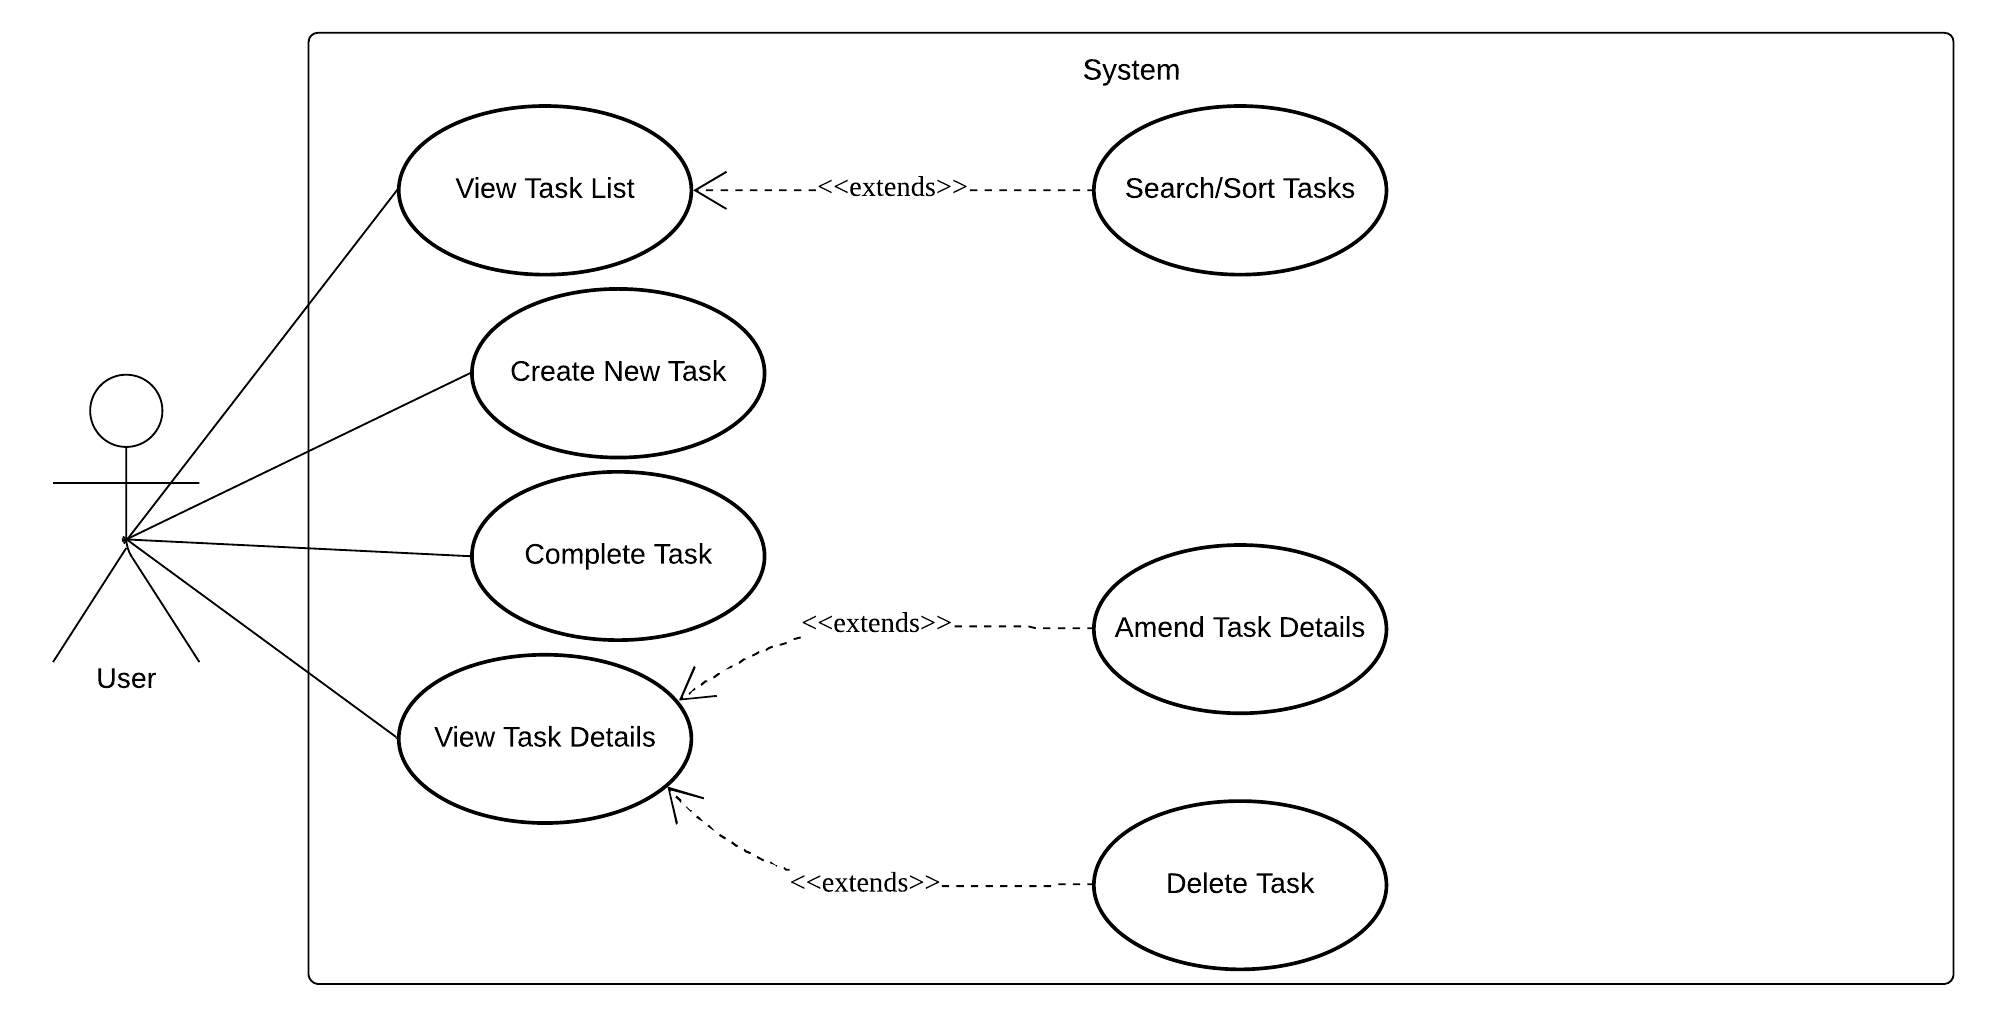
\includegraphics[width=\linewidth]{usecase.png}
	\caption{Use Case Diagram}
\end{figure}

\begin{figure}[h]
	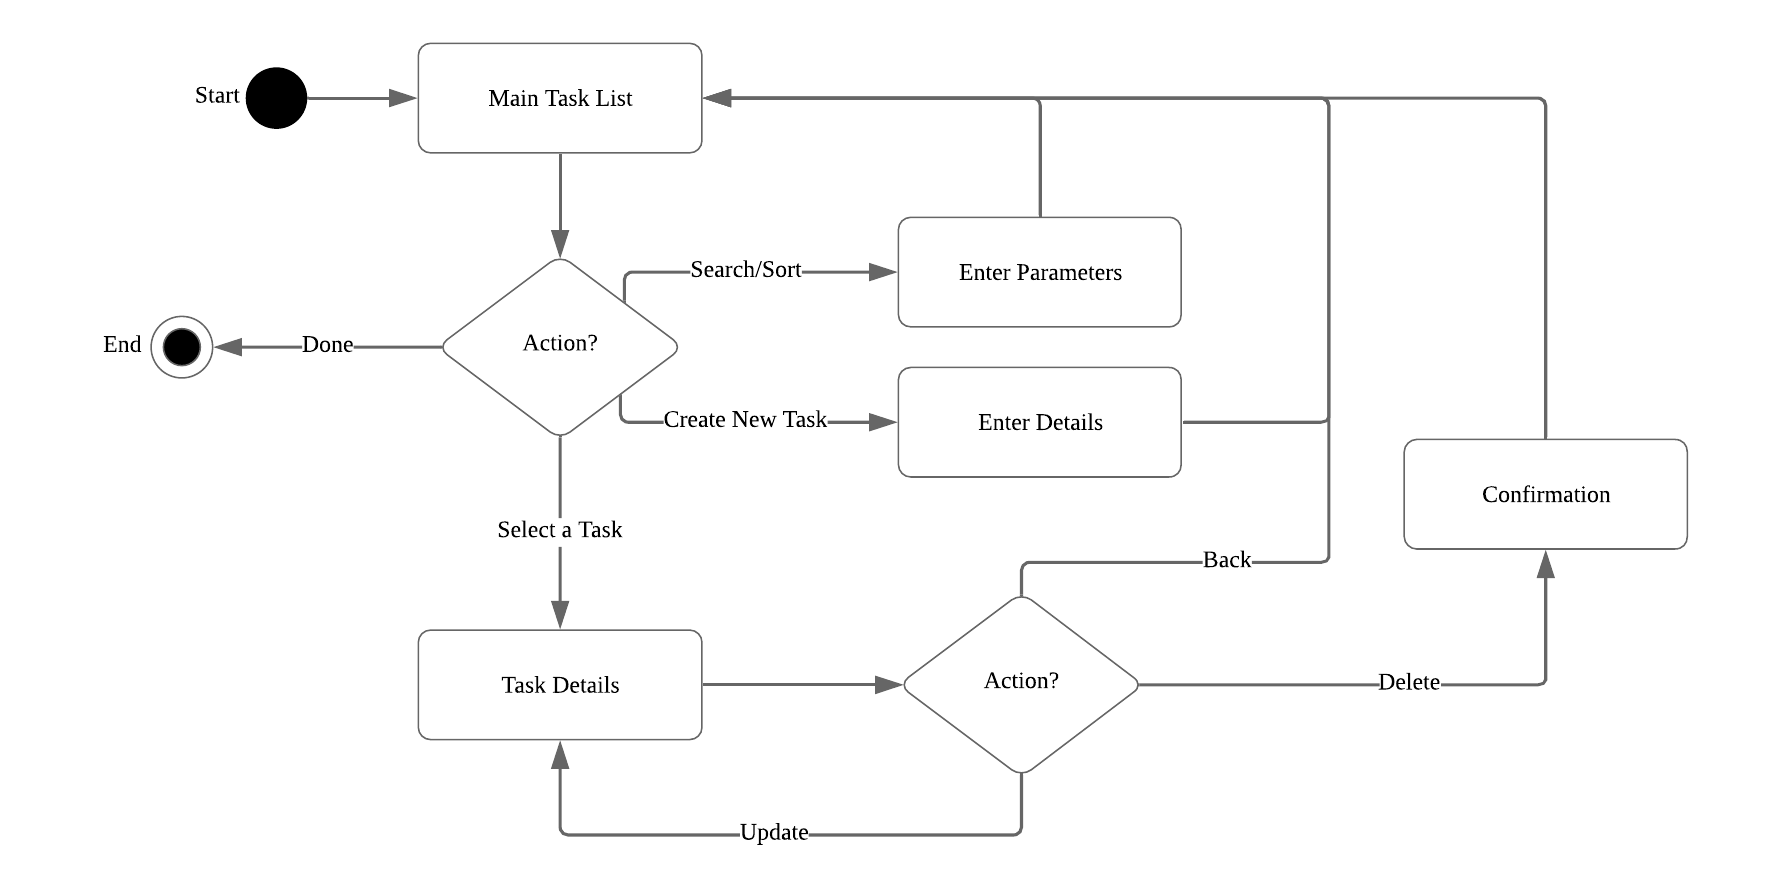
\includegraphics[width=\linewidth]{activity.png}
	\caption{Activity Diagram}
\end{figure}

	\newpage
	\section{Extra Stuff}
\setlength{\parindent}{0pt}
\setlength{\parskip}{1em}
		\subsection{Inexperience}
Having no prior experience in these technologies makes this assignment rather challenging, as I am not familiar with the styles and conventions of the specific languages. Although I expect to pick up on these conventions as I learn, the final project code will likely not conform to the exact standards due to beginner mistakes and gotchas. 

Where appropriate, I try to apply software engineering concepts in this project (e.g. the diagrams in the previous page). However, given that I have \textit{not} actually taken CS2103/T yet, some of these may not be 100\% correct/accurate. I would hence like to seek magnanimous grading in this aspect.
		\subsection{Setup}
In some of my past projects, simply setting up the development environment was half the battle. Broken dependencies and outdated documentation sometimes makes for an infuriating experience before any code is even written. Guides for Rails seem to rely heavily on command-line tools, and most prefer a Linux environment over anything else. Hence, to minimize the amount of time wasted troubleshooting the development environment, I decided to use an Ubuntu Virtual Machine to test and develop the project.

The advantage of a VM is the ability to save and restore snapshots of the environment, much like Git does for code. If something in the environment breaks later on, the environment can be rolled back to the last working snapshot while the latest code can be retrieved via GitHub. All in all, installing all the dependencies was done smoothly by following the shell commands in the provided guides.
		\subsection{Next Steps}
The next step from here will be to actually start coding the project. I intend to set up the backend (e.g. database) first, so that the frontend features can immediately be linked to the backend as they are developed. Once a minimum viable product has been achieved, then additional features and deliverables can be made, such as third-party hosting and the user manual.

\end{document}